\documentclass[12pt]{article}
\usepackage{setspace, amsmath, mathdots, amssymb, graphicx, multirow, gensymb, slashbox}
\usepackage[margin=1.5in]{geometry}
\onehalfspacing

\begin{document}
\noindent STA 250 Homework 1 \newline Yichuan Wang \newline \newline
\textbf{Problem 1} \newline
(a) Based on the characterization of stationary distribution, we have, for Gibbs sampler, 
\begin{center}
	$\pi(\mathbf{x}^{(t+1)}) = \int \pi(\mathbf{x}^{(t)})k(\mathbf{x}^{(t+1)}, \mathbf{x}^{(t)})d\mathbf{x}^{(t)}$
\end{center}
We may assume the Markov chain generated by Gibbs sampler is ergodic so that as $t \rightarrow \infty$, $P(X^{(t)} = \mathbf{x}) \rightarrow \pi(\mathbf x)$. The transitional kernel here is $p(x_1^{(t+1)}|x_2^{(t)})p(x_2^{(t+1)}|x_1^{(t+1)})$. Then we get
\begin{align*}
	\pi(\mathbf{x}^{(t+1)}) &=  \int \int \pi(\mathbf{x}^{(t)})p(x_1^{(t+1)}|x_2^{(t)})p(x_2^{(t+1)}|x_1^{(t+1)})dx_1^{(t)} dx_2^{(t)} \\
	&= p(x_2^{(t+1)}|x_1^{(t+1)})  \int p(x_1^{(t+1)}|x_2^{(t)}) \int \pi(\mathbf{x}^{(t)}) dx_1^{(t)} dx_2^{(t)} \\
	&= p(x_2^{(t+1)}|x_1^{(t+1)})  \int p(x_1^{(t+1)}|x_2^{(t)}) p(x_2^{(t)}) dx_2^{(t)} \\
	&= p(x_2^{(t+1)}|x_1^{(t+1)}) p(x_1^{(t+1)}) \\
	&= p(\mathbf{x})
\end{align*}
So the stationary distribution is the desired target distribution. \newline
(b) In the p-dimensional case, we have for the kernel distribution
\begin{align*}
	k(\mathbf{x}^{(t+1)}, \mathbf{x}^{(t)}) =\ &p(x_1^{(t+1)}|x_2^{(t)}, \cdots, x_p^{(t)})p(x_2^{(t+1)}|x_1^{(t+1)}, x_3^{(t)}, \cdots, x_p^{(t)}) 		\cdots \\
	&p(x_p^{(t+1)}|x_1^{(t+1)}, \cdots, x_{p-1}^{(t+1)})
\end{align*}
Similar to part (a) we have for the stationary distribution of Gibbs sampler components $\pi(\mathbf{x}^{(t+1)}) = \int \pi(\mathbf{x}^{(t)})k(\mathbf{x}^{(t+1)}, \mathbf{x}^{(t)})d\mathbf{x}^{(t)}$, where $\mathbf{x}^{(t)}, \mathbf{x}^{(t+1)} \in \mathbb{R}^p$. Again we may assume the Markov chain is ergodic so as $t \rightarrow \infty$, $P(X^{(t)} = \mathbf{x}) \rightarrow \pi(\mathbf x)$. Carrying out the integration in the same fashion as for bivariate case in part (a), eventually after integrating out p integrals, we will get that
\begin{align*}
	\pi(\mathbf{x}^{(t+1)}) = p(\mathbf x)
\end{align*}
So the same conclusion holds for p-dimentional case.
\newline
\newline
\textbf{Problem 2} \newline
(i)
\begin{center}
	$Y_i|\beta \sim \text{Binomial}(m_i, \text{logit}^{-1}(x_i^T\beta)), \beta \in \mathbb{R}^p$
\end{center}
So we have
\begin{align*}
	p(y_i|\beta) &= {m_i \choose y_i}(\frac{e^{x_i^T\beta}}{1+e^{x_i^T\beta}})^{y_i}(1 - \frac{e^{x_i^T\beta}}{1+e^{x_i^T\beta}})^{m_i - y_i} \\
	&= {m_i \choose y_i}\frac{e^{(x_i^T\beta)y_i}}{(1+e^{x_i^T\beta})^{m_i}}
\end{align*}
Then
\begin{align*}
	p(\mathbf{y}|\beta) \propto \frac{\exp({\sum_{i=1}^n(x_i^T\beta)y_i})}{\prod_{i=1}^n (1+e^{x_i^T\beta})^{m_i}}
\end{align*}
and
\begin{align*}
	p(\beta) \propto \exp[-\frac{1}{2}(\beta - \mu_0)^T \Sigma_0^{-1} (\beta - \mu_0)]
\end{align*}
So the posterior is, up to proportionality
\begin{align*}
	p(\beta|\mathbf{y}) \propto \frac{\exp[\sum_{i=1}^n(x_i^T\beta)y_i - \frac{1}{2}(\beta - \mu_0)^T \Sigma_0^{-1} (\beta - \mu_0)]}{\prod_{i=1}^n (1+e^{x_i^T\beta})^{m_i}}
\end{align*}
We may take logarithm of the proportional posterior for calculation, which is
\begin{align*}
	\sum_{i=1}^n(x_i^T\beta)y_i - \frac{1}{2}(\beta - \mu_0)^T \Sigma_0^{-1} (\beta - \mu_0) - \sum_{i=1}^n m_i \log(1+e^{x_i^T\beta})
\end{align*}
(ii) In this problem, I used the Metropolis-Hastings-within-Gibbs to generate the Markov chain for posterior distribution. The proposal distribution was
\begin{align*}
	\begin{pmatrix} \beta_0^{(t)} \\ \beta_1^{(t)} \end{pmatrix} | \begin{pmatrix} \beta_0^{(t-1)} \\ \beta_1^{(t-1)} \end{pmatrix} \sim 					N(\begin{pmatrix} \beta_0^{(t-1)} \\ \beta_1^{(t-1)} \end{pmatrix}, \begin{pmatrix} v_0^2 & 0 \\ 0 & v_1^2 \end{pmatrix})
\end{align*}
The algorithm was performed as the following: \newline
(1) Set initial values $\beta_0^{(0)} = 0, \beta_1^{(0)} = 0, t = 0, v_0 = v_1 = 1$. \newline
(2) Let $\beta_0^{(t+1)} = \beta_0^{(t)}, \beta_1^{(t+1)} = \beta_1^{(t)}$, sample $\beta_0^{(t+1)}$ from $N(\beta_0^{(t)}, v_0)$. \newline
(3) Compute the logarithm posterior of $\begin{pmatrix} \beta_0^{(t+1)} \\ \beta_1^{(t+1)} \end{pmatrix} | \begin{pmatrix} \beta_0^{(t)} \\ \beta_1^{(t)} \end{pmatrix}$, $\log \pi(\beta^{(t+1)}|\beta^{(t)})$, as well as the logarithm posterior of $\begin{pmatrix} \beta_0^{(t)} \\ \beta_1^{(t)} \end{pmatrix} | \begin{pmatrix} \beta_0^{(t+1)} \\ \beta_1^{(t+1)} \end{pmatrix}$, $\log \pi(\beta^{(t)}|\beta^{(t+1)})$. \newline
(4) Since we are using a symmetric proposal distribution, we have $\log\alpha = \log \pi(\beta^{(t)}|\beta^{(t-1)}) - \log \pi(\beta^{(t-1)}|\beta^{(t)})$.
(5) According to MH algorithm, when $\alpha > 1$, we always accept sample; when $\alpha < 1$, we accept with probability $\alpha$. \newline
(6) After updating (accepting or rejecting sample) $\beta_0^{(t+1)}$, we sample $\beta_1^{(t+1)}$ from $N(\beta_1^{(t)}, v_1)$ and repeat steps (3) to (5) to update it. \newline
(7) Set $t = t+1$, repeat steps (2) through (6) until desired iterations or convergence. \newline
For each dataset, 10000 iterations were executed and the first 1000 were considered as "burnin" period, during which retuning was performed at every $100^{th}$ iteration: if the acceptance rate for either parameter is too low (less than 20\%), the standard deviation $v_j$ would be divided by 1.1; if the rate is too high (greater than 60\%), the variance would be multiplied by 1.1. \newline
(iii) The following table and graph display the coverage property based on results from Gauss:
\begin{table}[ht]
\centering
\begin{tabular}{rrr}
  \hline
 & beta\_0 & beta\_1 \\ 
  \hline
p\_01 & 0.01 & 0.01 \\ 
  p\_05 & 0.07 & 0.03 \\ 
  p\_10 & 0.10 & 0.06 \\ 
  p\_25 & 0.27 & 0.20 \\ 
  p\_50 & 0.52 & 0.48 \\ 
  p\_75 & 0.76 & 0.77 \\ 
  p\_90 & 0.92 & 0.88 \\ 
  p\_95 & 0.94 & 0.95 \\ 
  p\_99 & 0.99 & 0.99 \\ 
   \hline
\end{tabular}
\end{table}
\newline
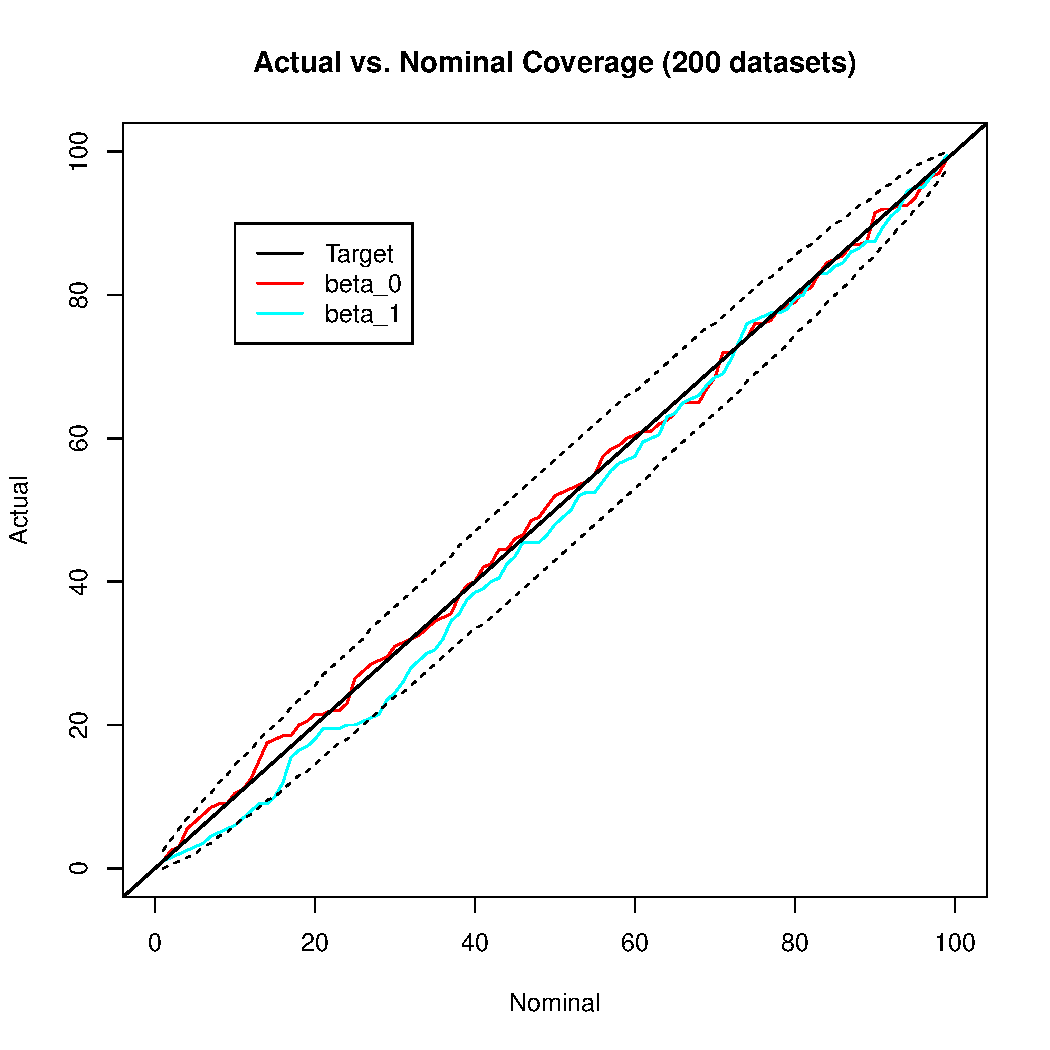
\includegraphics[width=\textwidth]{coverage_line_plot.pdf}
\newline
It seems that the result from this algorithm is satisfactory since the credible intervals cover the target/true values of $\beta$ parameters, with which the datasets were simulated.
\newline \newline
\textbf{Problem 3} \newline
(a) Similar to what I did in problem 2, MH-within-Gibbs algorithm was used to fit the logistic regression model after converting the response variable into a numerical one, $y$, with "M" set to be 1 and "B" to be 0. In total 100000 iterations were executed with the first 10000 being the burnin and retune period. For each covariate, the 95\% central credible interval was obtained:
\begin{table}[ht]
\centering
\begin{tabular}{rrrrrrrrrrrr}
  \hline
 $\beta_j$ & 0 & 1 & 2 & 3 & 4 & 5 & 6 & 7 & 8 & 9 & 10 \\ 
  \hline
2.5\% & -0.90 & 1.03 & -2.30 & 0.35 & -0.64 & -1.82 & -38.12 & -28.01 & 0.17 & -0.21 & 1.19 \\ 
  97.5\% & 1.46 & 24.15 & 2.29 & 5.38 & 2.45 & 0.85 & 17.80 & 36.42 & 2.21 & 1.18 & 2.52 \\ 
   \hline
\end{tabular}
\end{table}
\newline
Note that in order to simplify the problem, standardization was performed on each covariate before the sampling algorithm. \newline
(b) The autocorrelation of lag-1 was calculated for each covariate
\begin{table}[ht]
\centering
\begin{tabular}{rrrrrrrrrrrr}
  \hline
 $\beta_j$ & 0 & 1 & 2 & 3 & 4 & 5 & 6 & 7 & 8 & 9 & 10 \\ 
  \hline
$\rho_1$ & 0.955 & 0.997 & 0.973 & 0.940 & 0.929 & 0.966 & 0.999 & 1.000 & 0.926 & 0.828 & 0.850 \\ 
   \hline
\end{tabular}
\end{table}
 \newline
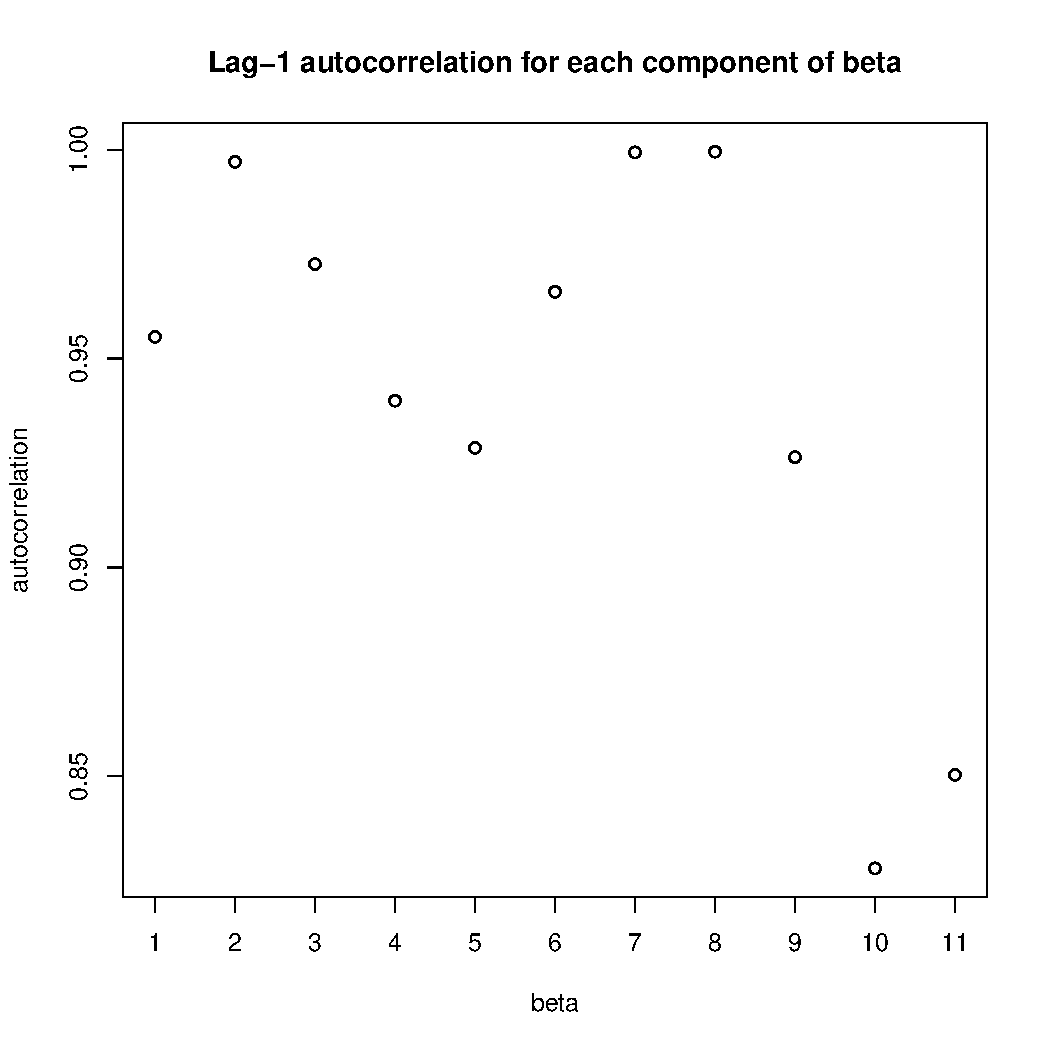
\includegraphics[width=\textwidth]{pb3_acf_plot.pdf} \newline
(c) Based on the credible intervals of parameters, covariates $x_1, x_3, x_8, x_{10}$ seem to be related to cancer diagnosis. They represent radius (mean of distances from center to points on the perimeter), perimeter, concave points (number of concave portions of the contour) and  fractal dimension ("coastline approximation" - 1) respectively. \newline
(d) For the posterior predictive check, 10000 samples were generated from the posterior distribution of covariates and rbinom() function was used to obtain a predictive numerical vector, $y^*_k$ from each sample, for $k = 1, \cdots, 10000$. Then the mean of each predicted $y^*_k$ with the histogram plotted below, the red vertical line represents the mean of the original diagnosis vector $y$. \newline
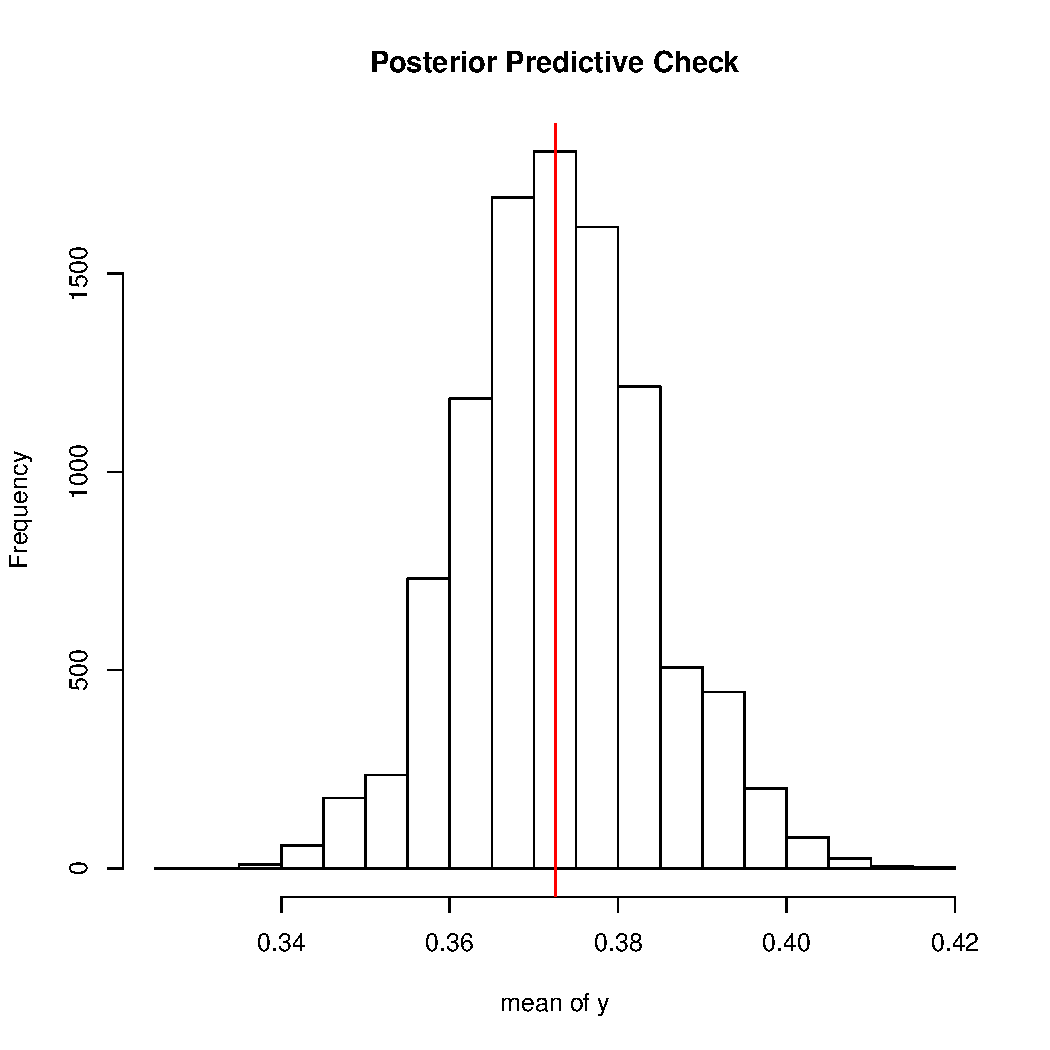
\includegraphics[width=\textwidth]{pb3_check.pdf} \newline
The histogram from posterior predictive check showed that the simulated diagnosis is somewhat similar to the original one.\newline
(e) The model seems to be a reasonable fit to the data. Because the posterior predictive check returned a good result compared with the original data, i.e. the diagnoses. Also it showed that only a few of all the covariates, 4 out of 11, are more related to the cancer diagnosis, providing a plausible guess for variable selection.
\end{document}